\chapter{Meshing}
\label{chap:meshing}

\framepart{Outline}
This chapter is devoted to the discussion of mesh creation. We review the basic commands 
and show a series of examples of one, two or three dimensional bodies embedded 
in a two or three dimensional space. 

\section{General settings}

The first setting defines the dimensions of the working space and 
the coordinate system.
These general settings are defined through the \texttt{opti} operator.  
\dindex{opti[on]}{settings}

\begin{castemcom}
This command defines a two dimensional working space 
and quadrangular elements as the basic bricks for the 
mesh. However simpler elements like points, segments or 
triangular will also be created by the called operators.    
\end{castemcom}
\begin{castemlines}
\begin{verbatim}
opti dime 2 elem QUA4; 
\end{verbatim}
\end{castemlines}

\FloatBarrier

The finite element theory uses fields defining their values 
at specific points of elements. Elements are simple geometrical figures, i.e. 
triangles, quadrangles, \ldots, cubes, pyramids, \ldots. The set of elements 
will represent the continuous body and the associated data structures 
are given by the (i) nodal coordinates and (ii) the list of connectivities 
defining the set of nodes for each element.

Depending on the type of the object we can define different types of associated 
meshes: points, lines, surfaces or volumes. 

\begin{gbox}{Mesh Options}
\begin{tabular}{ll}
\texttt{opti \ldots;} & command for defining general settings \\
\texttt{dime} & dimension of the working space \\
\texttt{elem} & basic element type for the mesh \\
\end{tabular}
\end{gbox}

\section{Examples of 2D mesh creation}

\subsection*{Quadrangular plate with a hole}

\begin{castemcom}
The operator \texttt{opti} does not create objects, but defines the general settings of the 
computation by using a series of key-words. Here we define a two \texttt{dime[nsion]}-al 
space and by default a plane strain situation. The basic element is chosen 
by \texttt{elem QUA4} to be the linear isoparametric quadrangle. 

The corners of the mesh are defined using their coordinates 
values as functions of the size \texttt{ldom} of the domain 
and of the radius  \texttt{r} of the hole
(see figure~\ref{fig:castem:trou})

\end{castemcom}
\begin{castemlines}
\begin{verbatim}
opti dime 2 echo 1 elem QUA4; 

ldom = 1.; r = 0.1; 

p1 = 0. 0.; 
p2 = ldom 0.; 
p3 = ldom ldom; 
p4 = 0. ldom; 

a2 = r 0.; 
a4 = 0. r; 
a3 = (r/1.4142) (r/1.4142); 
\end{verbatim}
\end{castemlines}

\begin{castemcom}
The operators \texttt{droi[te]} and \texttt{cerc[le]} build the straight and
circular segments of the contour of the mesh. The number of elements on each
segment is given by the parameters \texttt{nel} and \texttt{nel\_bis}, and
the size of the first and of the last element is specified after the keywords
\texttt{dini} and \texttt{dfin}. A \emph{negative} element count, as in
\texttt{nel\_bis}, is what tells the operator to grade the element size
between those two values -- which is how the mesh is refined near the hole,
where the stress gradient is.

The mesh \texttt{dom} is built with \texttt{dall[er]}, initially in two
parts which are then joined with \texttt{et}. \texttt{inve[rser]} reverses
the order in which the nodes of a contour are traversed; \texttt{dall[er]}
needs its four sides given head to tail, so some of them have to be reversed
to obtain a correct mesh. If \texttt{dall} refuses a contour, this is almost
always why.

Finally the mesh is displayed with \texttt{trac[er]}. 
\dindex{droi[te]}{line}
\dindex{cerc[le]}{circle}
\dindex{dall[er]}{tiling 2D}
\dindex{inve[rser]}{change order}
\dindex{et}{and}

\end{castemcom}
\begin{castemlines}
\begin{verbatim}
  nel = 10;  nel_bis = -20;

  d12 = droite  nel_bis  a2 p2 
             dini 0.002 dfin 0.15 ;
  d23 = droite nel p2 p3;
  d34 = droite nel p3 p4;
  d41 = droite nel_bis p4 a4 
             dini 0.15 dfin 0.002 ;
  bis = droite nel_bis a3 p3 
             dini 0.003 dfin 0.22 ;
  arc23 = cerc nel a2 p1 a3;
  arc34 = cerc nel a3 p1 a4;   

  dom1 = dall 
    d12 d23 (inve bis) (inve arc23);
  dom2 = dall (inve d41) (inve d34) 
              (inve bis) arc34;
  dom  = dom1 et dom2;
  
  trac dom;

\end{verbatim}
\end{castemlines}

\begin{gbox}{Operators for 2D mesh creation}
\begin{tabular}{ll}
\texttt{droi[te]} & creates a straight line \\
\texttt{cerc[le]} & creates circle defined by the center and two of its points \\
\texttt{cer3} & creates circle defined by three of its points \\
\texttt{para[bolic]} & creates a parabolic arc \\
\texttt{cubp, cubt} & create cubic  \\[2.mm]
\texttt{dall[er]} & 2D tiling of a curved quadrangular  \\
\texttt{pav[er]} &  3D tiling a curved cubic envelope   \\
\texttt{surf[ace]} & creates a surface by filling its closed boundary \\
\texttt{tran[slation]} & creates a surface by translation \\
   & of a line along a given vector  \\
\texttt{rota[tion]} & creates a surface by rotation \\
   & of a line around a point or a line  \\
\end{tabular}
\end{gbox}


\begin{castemcom}
In order to illustrate another technique for constructing a surface, We first 
recover the boundary of the domain \texttt{dom} using the \texttt{cont[our]} 
operator and we then proceed by refilling the closed boundary using the 
\texttt{surf[ace]} command.

One can remark that the new domain is irregular and that triangles have
been used in its creation in spite of the \texttt{QUA4} element setting 
at the beginning of the file.

\index{contour@ \texttt{cont[our]}, boundary line of a surface}
\index{surface@ \texttt{surf[ace]}, meshes a closed line}

      
\end{castemcom}
\begin{castemlines}
\begin{verbatim}
 
  domcon = contour dom;
  dombis = surf domcon;
 
  trace dombis;
  
\end{verbatim}
\end{castemlines}

\begin{castemcom}
A domain can also be created by translation of a line along 
a vector. The example translates the arc \texttt{arc23} 
along the \texttt{(0. r)} vector. The vector is not only used to 
define a direction but also the length of the translation. 

The four sides of the new domain can be recovered by applying the
\texttt{face} (side) command to the domain, numbered in the order in which
the translation generated them. Clicking the \texttt{Qualification} button in
the trace window shows which face number corresponds to which edge, which is
how you find out what to name \texttt{arc23b}.
\end{castemcom}
\begin{castemlines}
\begin{verbatim}
 
  dom23 = arc23 tran nel (0. r);
  arc23b = dom23 face 3;
  
  trace dom23; 
 
\end{verbatim}
\end{castemlines}

\begin{figure}
\centerline{
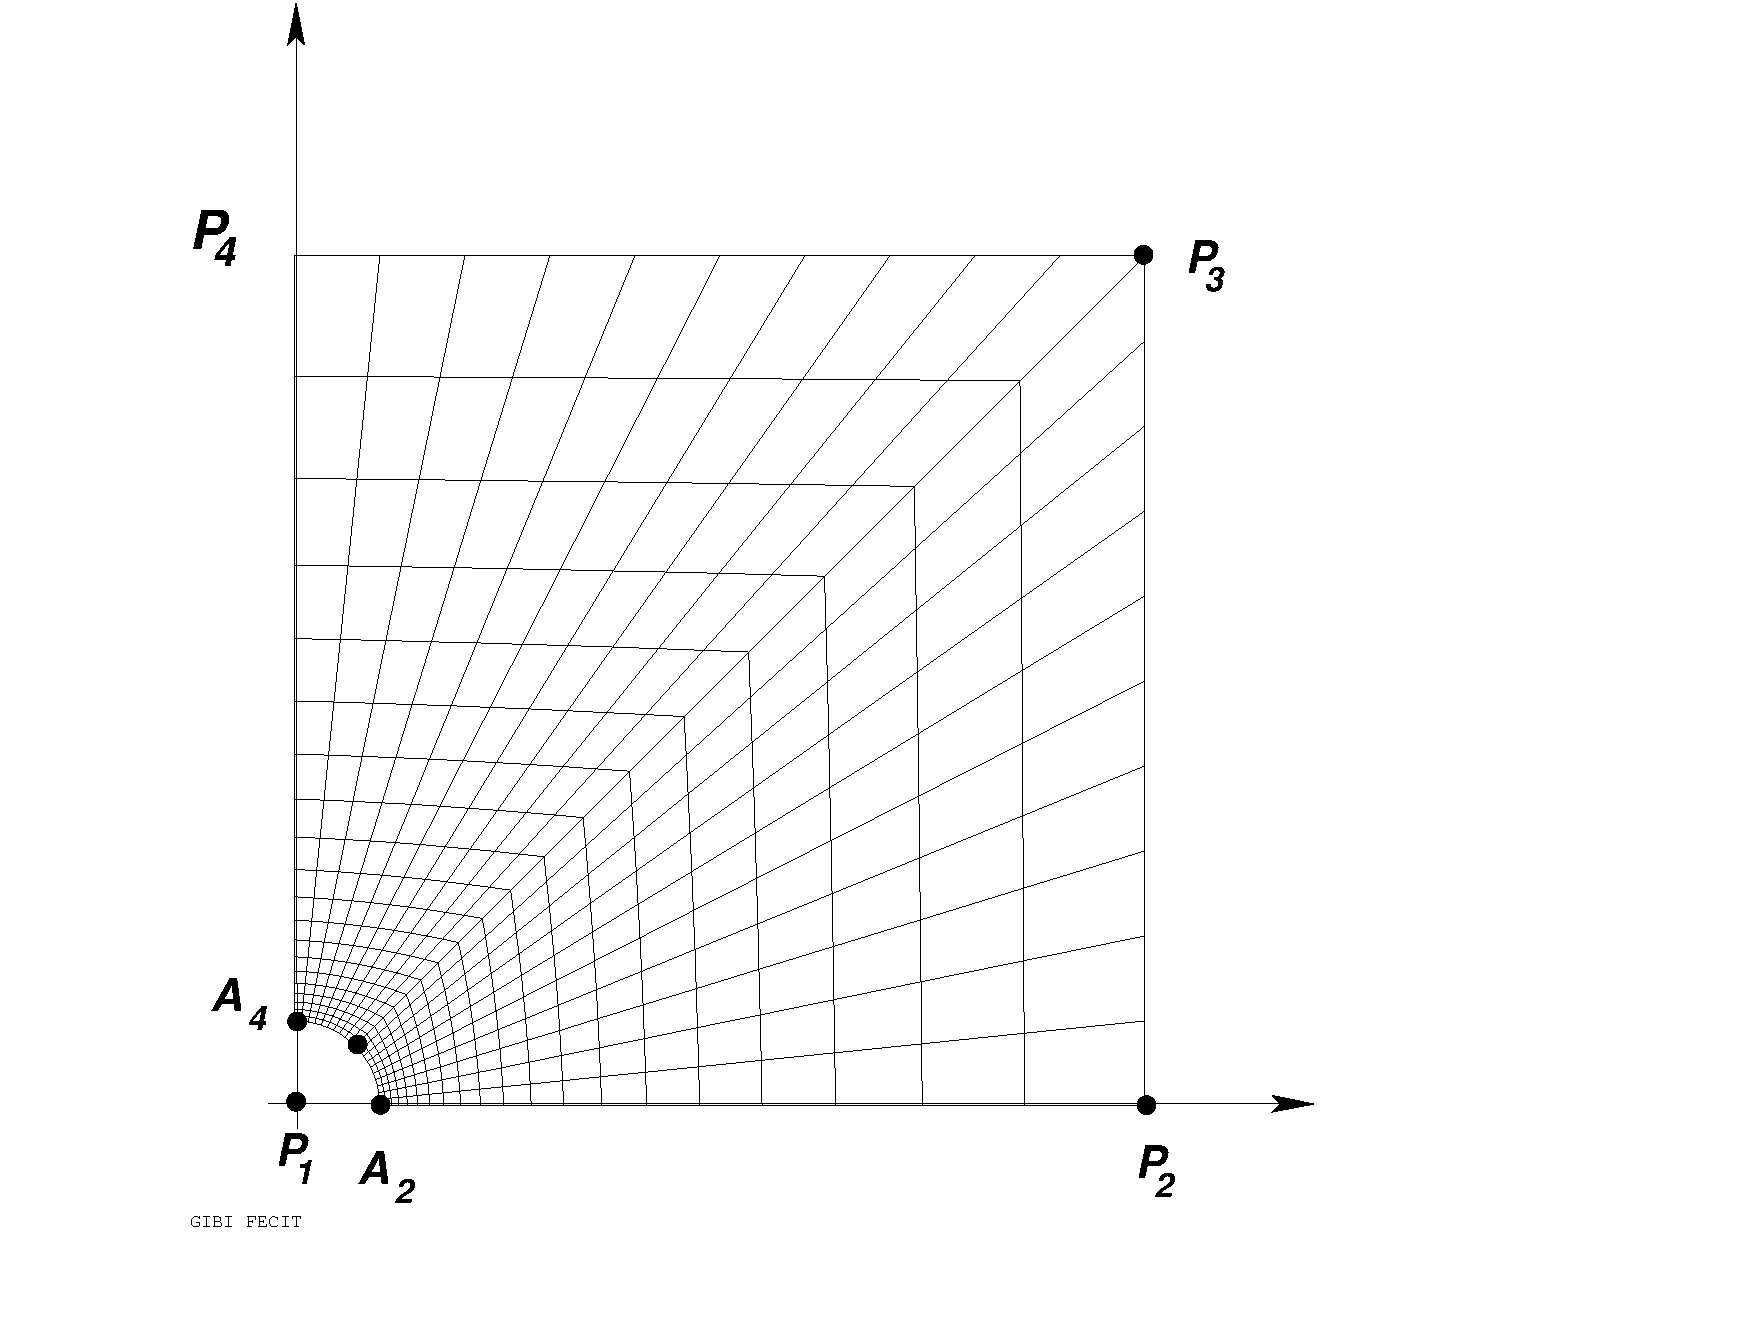
\includegraphics[height=5.cm]{./FIG/trou}
}
\caption{The quarter of a plate with a hole, in tension}
\label{fig:castem:trou}
\end{figure}

\begin{gbox}{Operators for 2D mesh creation}
\begin{tabular}{ll}
\texttt{cont[our]} & recovers the boundary of a domain \\
\texttt{syme[trie]} & creates the symmetric of a given mesh   \\
\texttt{tour[ner]} & creates  a new rotated mesh from of a given one   \\
\texttt{plus} & creates  a new  mesh by adding a displacement to a given mesh   \\
\texttt{elim[iner]} & eliminates nodes with close coordinates \\
\texttt{dedo[ublement]} & doubles existing nodes (the opposite of \texttt{elim[iner]}) \\
\texttt{poin[t]} & selects a set nodes of a given mesh  \\
\texttt{elem[ent]} & selects elements of a given mesh  \\
\texttt{face} & selects the n-th face of a mesh in 2D or 3D  \\
\end{tabular}
\end{gbox}

\begin{castemcom}
The complete geometry of the quadrangular plate with the 
hole in the center can simply be created by completing 
the geometry through symmetry (operator \texttt{syme[trie]}). 

A series of geometrical points are now represented through 
different nodes, which can be shrunk into one unique node 
using the \texttt{elim[iner]} operator. The real number 
at the end of the last command is the tolerance, defining 
the neighborhood for which nodes are reduced to one 
single node.
\dindex{elim[iner]}{merge close nodes}
\index{dedoubler @ \texttt{dedo[ubler]}}

It is worth noticing that an inverse command equally 
exists \texttt{dedo[ubler]} which creates additional nodes (doubles) 
for existing nodes. An example of application is the 
creation of cracks. 

\dindex{elim[iner]}{merge close nodes}

\end{castemcom}
\begin{castemlines}
\begin{verbatim}
 
quart2 = dom syme 'DROIT' p1 p4;
half = (dom et quart2) syme 'DROIT' p1 p2;

plate = elim (dom et quart2 et half) 0.001;

\end{verbatim}
\end{castemlines}

A difficulty with the new geometry \texttt{plate} is that its 
points, border lines and nodes, do not have a distinct name. 
Surely, one can address these objects by their node or element
number, but this will not provide an intrinsic solution as 
is might change with a new parametrization of the geometry 
or simply a new run of the program. The problem is solved 
by the \texttt{poin[t]} and \texttt{elem[ent]} operators as
illustrated in the next lines.
 
\begin{castemcom}
The \texttt{poin[t]} command will select the points of the 
contour of the plate, \texttt{cont plate}, lying within 
$0.001$ of the line (fr. \texttt{'DROITE'} ) 
defined by the points 
$(0., \, -l_{dom})$ and $(1., \, -l_{dom})$.

Next in a similar way, the \texttt{elem[ent]} command will 
select the elements of contour of the plate, 
\texttt{cont plate}, lying (fr. \texttt{'APPUYE'} ) 
strictly (fr. \texttt{'STRICTEMENT'} ) on the set points 
\texttt{poi\_line}.
\dindex{poin[t]}{select points or nodes}
\dindex{elem[ent]}{select elements}

The result is finally plotted using \texttt{trac[er]}. 
One can remark that the colour of the points has been 
changed into green (fr. \texttt{vert}) for a better  
display.

\end{castemcom}
\begin{castemlines}
\begin{verbatim}

poi_line = (cont plate) poin 'DROITE' 
        (0. (-1. * ldom))
        (1. (-1. * ldom)) 0.001;
	       
ele_line = (cont plate) elem
    'APPUYE' 'STRICTEMENT' poi_line;
 
trace ((cont plate)
       et (poi_line coul vert)
       et (ele_line coul rouge));
\end{verbatim}
\end{castemlines}

\section{Example of a 3D mesh creation}
\label{sec:mesh:3d}

Most of the commands presented in the preceding section will 
equally function in a three dimensional environment, creating 
the embedded points, lines or surfaces. We shall briefly illustrate 
one of the construction commands.   

\begin{castemcom}

The passage from two to three dimensions can be done 
in the middle of a program, if so the third coordinate 
of all existing objects will automatically be 
set to $0.$. This can readily be observed by plotting 
the third coordinate of the \texttt{plate}.  

The two dimensional surface: \texttt{plate},
can be extruded using the \texttt{volu[me]} 
command into a three dimensional cube.  

The \texttt{enve[loppe]} command recovers the 
boundary of the mesh exactly as \texttt{cont[our]} 
in the two dimensional case.

The extremal sections of the extruded volume 
can be recovered as the $1$ and $2$ face of the \texttt{cube},
while the cylindrical surface of the extrusion will form 
the $3$ face.  

\index{face@ \texttt{face} of a volume}
\index{envelope@ \texttt{enve[loppe]}, boundary surface of a volume}

\index{plus@ \texttt{plus}, new mesh by a adding a displacement}

\end{castemcom}
\begin{castemlines}
\begin{verbatim}

opti dime 3 elem cub8;

trace plate (plate coor 3);

cube = plate volu tran nel (0. 0. ldom);

trace cach cube;

trace cach (enve cube);

trace cach (cube face 1);
trace cach (cube face 2);
trace cach (cube face 3);

\end{verbatim}
\end{castemlines}


\section{Surfaces of revolution and ruled surfaces}
\label{sec:mesh:revolution}

\cindex{surface of revolution}\cindex{ruled surface}%
\cindex{cylindrical shell}\cindex{hyperbolic paraboloid}%
\cindex{cooling tower}%
Two families of surface deserve their own section, because they are the
geometries the eigenvalue computations of chapter~\ref{chap:eigen} are built
on and because each is produced by a single operator: a \emph{surface of
revolution}, made by rotating a line about an axis, and a \emph{ruled
surface}, made by sweeping a straight segment between two guide curves.

\subsection*{A cylindrical shell}

The thin cylinder is the standard specimen for both vibration and buckling: it
has analytical solutions, and it buckles in a pattern of circumferential
lobes that is easy to see.

\begin{castemcom}
\op{rota} \dindex{rota[tion]}{surface of revolution}
\dindex{tour[ner]}{rotate an existing object} sweeps a line about an
axis -- a point in 2D, two points defining the axis in 3D -- through a given
angle, and returns the surface it generates. Here the generating line is the
vertical segment \op{lgen} at radius $R$, swept through $360^{\circ}$ about
the $z$ axis. Note that it must not be called \op{gene}: an object whose
first four characters match an operator destroys that operator for the rest
of the session, and \op{gene} is one.

The angle is in degrees, and its sign sets the orientation of the generated
elements, which matters as soon as you apply a pressure or a contact
condition to the surface.

\medskip
A full revolution closes on itself, so the first and last nodes coincide
geometrically but are distinct objects: \op{elim} merges them. Forget it and
the cylinder is a rolled sheet with a seam, which shows up as a spurious
mode.
\end{castemcom}
\begin{castemlines}
\begin{verbatim}
opti dime 3 elem qua4;

rcyl = 0.5;  hcyl = 2.;
nh   = 20;   ncirc = 48;

* axis of revolution
pa = 0. 0. 0.;
pb = 0. 0. 1.;

* generating line, at radius rcyl
* (do not call it "gene": that would
*  shadow the GENE operator)
g1 = rcyl 0. 0.;
g2 = rcyl 0. hcyl;
lgen = droi nh g1 g2;

cyl = lgen rota ncirc 360. pa pb;
cyl = elim cyl 1.e-6;

* the two rims, for the boundary
* conditions
bas  = cyl poin 'PLAN' pa
       (1. 0. 0.) (0. 1. 0.) 1.e-4;
haut = cyl poin 'PLAN' g2
       (1. 0. hcyl) (0. 1. hcyl) 1.e-4;

trace cach cyl;
\end{verbatim}
\end{castemlines}

\dindex{cara[cteristiques]}{geometric characteristics}%
\cindex{shell thickness}%
\noindent A shell needs a thickness, which is not part of the mesh but of the
\emph{characteristics}: \op{cara mod 'EPAI' 0.002;}. That object is passed
alongside the material everywhere a stiffness is built -- see
chapter~\ref{chap:eigen}, where forgetting it is the commonest cause of a
buckling computation that returns nonsense.

\subsection*{A hyperbolic paraboloid}

The hyperbolic paraboloid is the shape of a natural-draught cooling tower. It
is doubly curved, yet it is a \emph{ruled} surface: it can be generated by a
straight line sliding between two circles of different radii, at different
heights, rotated relative to one another. That is why such towers can be built
from straight reinforcement.

\begin{castemcom}
\op{regl[er]} \dindex{regl[er]}{ruled surface} \sindex{gene[ratrice]}
builds the ruled surface joining two lines. The two lines must be \emph{of the same type}, have
\emph{the same number of elements}, and be described \emph{in the same
direction} -- the operator joins node $i$ of one to node $i$ of the other, so
if the surface comes out twisted into an hourglass, reverse one of them with
\op{inve}.

That twist is in fact the point here: the hyperbolic paraboloid is obtained
precisely by offsetting the two circles by a fraction of a turn. Rotating the
upper circle by $0^{\circ}$ gives a cone or a cylinder; the more you rotate
it, the more pronounced the waist.

\medskip
In 3D a full circle is built with the \texttt{'ROTA'} form of \op{cerc}:
rotate a starting point through $360^{\circ}$ about the axis given by two
points. The element count must be the same on both circles.
\end{castemcom}
\begin{castemlines}
\begin{verbatim}
opti dime 3 elem qua4;

rbas = 2.;  rhau = 1.6;  htot = 5.;
nc   = 48;  nv   = 20;
alph = 40.;

o1 = 0. 0. 0.;
o2 = 0. 0. htot;
za = 0. 0. 1.;

* lower circle: rotate a1 by 360
* about the axis o1-za
a1 = rbas 0. 0.;
c1 = cerc nc 'ROTA' 360. a1 o1 za;

* upper circle, offset by alph
b1 = rhau 0. htot;
b1 = b1 tour alph o2 za;
c2 = cerc nc 'ROTA' 360. b1 o2 za;

* a full circle closes on itself:
* merge the coincident end nodes,
* exactly as for the cylinder
c1 = elim c1 1.e-9;
c2 = elim c2 1.e-9;

* the ruled surface between them
tour1 = c1 regl nv c2;

trace cach tour1;
\end{verbatim}
\end{castemlines}

\noindent Setting \op{alph} to zero returns a truncated cone, which is a
useful check that the two circles are correctly matched before you introduce
the twist. The waist radius and its height follow from the geometry, and
comparing them with the computed mesh is the quickest way to confirm the
surface is the one you intended.

\begin{optable}{Surfaces of revolution and ruled surfaces}
rota[tion] & surface swept by rotating a line about a point (2D) or an axis
             (3D) \\
regl[er]   & ruled surface joining two lines of identical type and element
             count \\
tran[slation] & surface swept by translating a line along a vector \\
tour[ner]  & rotates an existing object (point, line, mesh) \\
volu[me]   & volume swept by a surface \\
gene[ratrice] & surface generated by translating one line parallel to another \\
cara       & geometric characteristics -- shell thickness, beam section \\
\end{optable}

%\subsection*{Rigid mouvements}

\section{Deformation of meshes}
\label{sec:mesh:deform}

A mesh can be deformed to create a new mesh just by adding 
a desired displacement field as illustrated 
in the next example.

\begin{castemcom}
We first extract the three coordinate fields of the plate,
and create the field: $u_z = x^2 + y^2$. The field 
will be labelled as the $z$ component of a displacement 
field after changing the name of its component 
from \texttt{'SCAL'} to \texttt{'UZ'}. 

The new mesh is simply created by adding the 
displacement to the initial mesh using the \texttt{plus}
command.

Finally results are plotted using \texttt{trace} 
after the colouring of the new mesh in red (fr. rouge) 
using \texttt{coul[eur]}

\end{castemcom}
\begin{castemlines}
\begin{verbatim}

xx yy zz = coor plate;

uuz = (xx * xx) + (yy * yy);
uuz = exco uuz 'SCAL' 'UZ';

pshell = plate plus uuz;

trace cach (plate et (pshell coul rouge));

\end{verbatim}
\end{castemlines}

\section{Meshes built elsewhere}

The import and export of meshes from and towards \texttt{Cast3M} 
is of importance for a series of practical applications. This topic 
is discussed in chapter~\ref{chap:importexport}.

\section{Numbers and measures for meshes}

\begin{castemcom}
The number of nodes and the number of elements of a mesh are simply 
recovered by applying the \texttt{nbno[euds]} \texttt{nbel[ements]}
operators.

\texttt{noeu[d]} permits to recover the geometrical point corresponding to 
the node of a mesh. Note however that node numbers change whenever the mesh
is regenerated, so \texttt{poin proc}, which looks a point up by its
coordinates, is the safer choice in a file you intend to re-run. 

\bigskip 

The area of the created meshes is computed 
by the \texttt{mesu[rer]} operator and the \texttt{surf[ace]} option. Other option,
\texttt{long[ueur]} (fr. length) and \texttt{volu[me]}
enable the computation of a length and a volume for 
one and respectively three dimensional objects.    

\index{mesurer@\texttt{mesu[rer]}, measures length, areas and volumes}
\index{nbno@\texttt{nbno[euds]}, computes the number of nodes}
\index{nbel@\texttt{nbel[ements]}, computes the number of elements}
 
\end{castemcom}
\begin{castemlines}
\begin{verbatim}

list (nbno pshell);
list (nbel pshell);

pp = pshell noeud 347;

* better: a geometric lookup, which
* survives a change of mesh
pp = pshell poin proc (0.5 0.5);
list (coor 1 pp);

list (mesu pshell 'SURF');


\end{verbatim}
\end{castemlines}

\begin{gbox}{Other operators for mesh manipulation}
\begin{tabular}{ll}
\texttt{nbel[ements]} & computes the number of elements of a mesh \\
\texttt{nbno[euds]} & computes the number of nodes of a mesh \\
\texttt{noeu[d]} &  defines a point using its nodal number \\[2.mm]
\texttt{mesu[rer]} & measures the length, surface or volume of a mesh \\
\end{tabular}
\end{gbox}

\framepart{Summary}

\begin{gbox*}
\begin{itemize}
  \item \textbf{A mesh is built upward}, from points to lines, then to
  surfaces and volumes, in two and in three dimensions. Each operator takes
  objects of the level below, which is why a careless point costs you the
  whole volume.
  \item \textbf{\op{opti dime} comes first.} The dimension of the working
  space and the element type are settings, not arguments, and they have to
  be set before anything is meshed.
  \item \textbf{Meshes put side by side are not joined.} Coincident points
  built twice stay two points until \op{elim} merges them, and a
  computation on an unmerged mesh runs happily and gives the wrong answer.
  \item \textbf{What is shown here is a small part of the whole.} The
  operators of this chapter cover a wide range of manipulations but by no
  means all of them; the rest is in the examples, the notices, and the
  reports on the \texttt{Cast3M} site.
\end{itemize}
\end{gbox*}

\framepart{Exercises}


\exercise{Hyperbolic paraboloid}

The hyperbolic paraboloid is a ruled surface (fr. surface r\'egl\'ee) generated by a line 
that pertains to two circles. This type of structures is used as a refrigeration 
tower for electricity generating plants. 

{\small \textit{Hint} use the \texttt{regl[er]} operator}





